\documentclass[12pt]{beamer}
\usetheme{CambridgeUS}
\usecolortheme{dolphin}
\usepackage[utf8]{inputenc}
\usepackage{amsmath}
\usepackage{amsfonts}
\usepackage{amssymb}
\usepackage{graphicx}
\usepackage{mathtools}
\usepackage{multimedia}
\usepackage[mathscr]{euscript}
\usepackage{xcolor}
\usepackage{algorithmicx}
\usepackage{algpseudocode}
\usepackage{setspace}

% Useful macro for circling numbers
\usepackage{tikz}
\newcommand*\circled[1]{\tikz[baseline=(char.base)]{
  \node[shape=circle,draw,inner sep=2pt] (char) {#1};}}

\DeclarePairedDelimiter{\abs}{\lvert}{\rvert}
\DeclarePairedDelimiter{\norm}{\lVert}{\rVert}

\newcommand{\R}{\mathbb{R}}
\newcommand{\C}{\mathbb{C}}
\newcommand{\Tau}{\mathcal{T}}
\newcommand{\AMz}{\underset{z}{arg\, min}}
\newcommand{\prox}{\text{prox}}

\newcommand{\worm}{WWWWWoooooooRRRRRmmmmmm}

\author[Rudy,Maass,Molloy,Mueller]{Samuel Rudy, Kelsey Maass, Riley Molloy, and Kevin Mueller}
\title[Denoising and Deblurring]{Image Denoising and Deblurring \\ \normalsize Applied Math 515 Final Project}
\setbeamercovered{transparent} 
%\institute{University of Washington} 
\date{March 12 2016} 
\subject{Amath 575} 

\iffalse
To d:
-Discuss different fidelity functions
-Discuss different regularizers
-Talk about optimization for wavelet method
-Talk about Frobenius norm denoising
-TV reg for denoising and deblurring
-Give lots of examples
-Talk about caveats of each method (parameters are a pain in the ass)
-bibliography
\fi

\begin{document}

% Title Page
\begin{frame}
\titlepage
\end{frame}

% Contents
\begin{frame}{Contents}
\tableofcontents
\end{frame}

% MOTIVATION
\section{Motivation}

% Cameraman example
\begin{frame}{Image Denoising and Deblurring}
\begin{center}
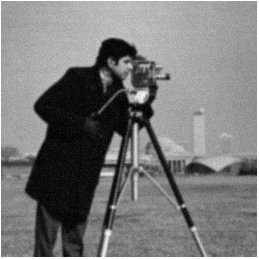
\includegraphics[scale=0.55]{../figures/bad_image.png}
\hspace{1 cm}
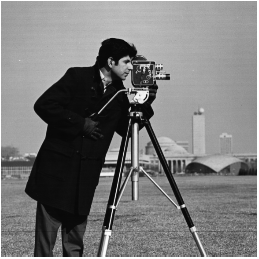
\includegraphics[scale=0.55]{../figures/good_image.png} 
\end{center}
\end{frame}

% Problem Formulation
\begin{frame}{Mathematical Formulation}
\begin{center}
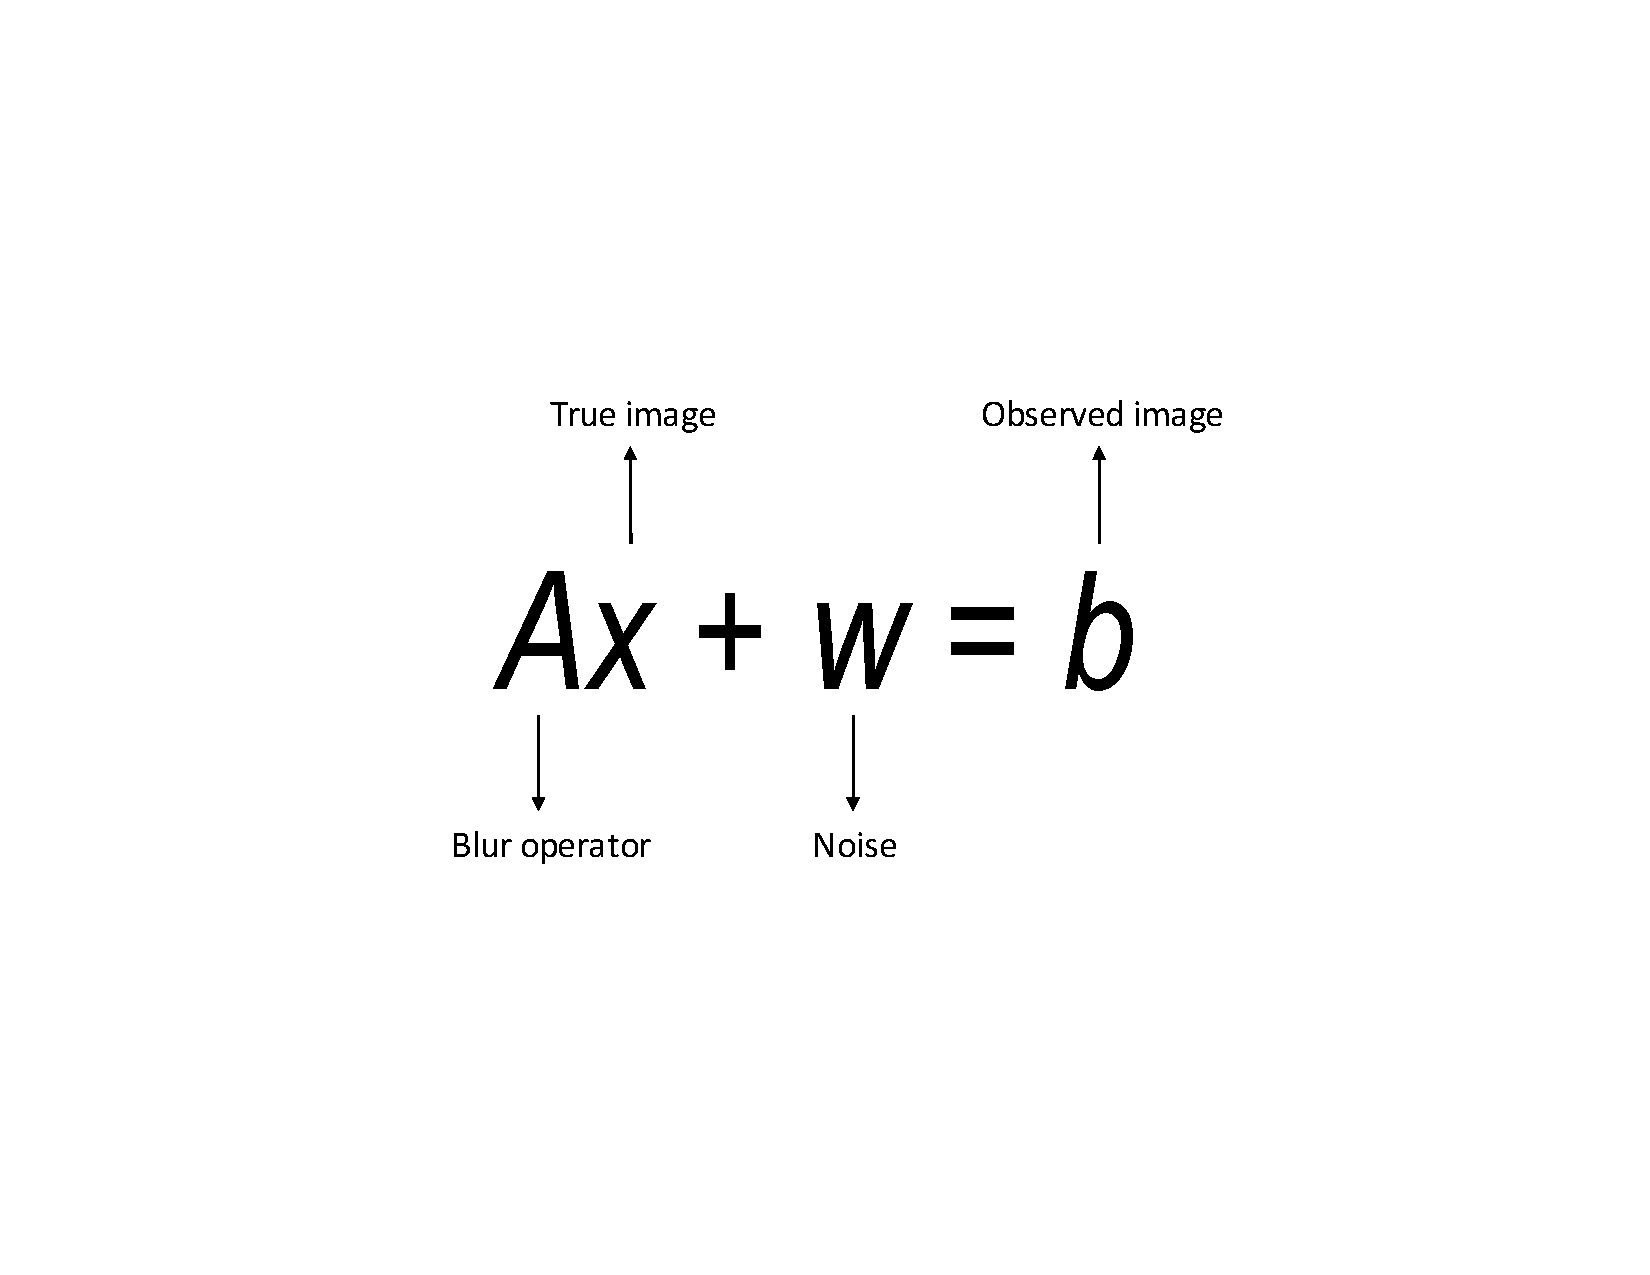
\includegraphics[scale=0.75]{../figures/linearModel}
\end{center}
\end{frame}
% add a slide to describe A and w

%\begin{frame}{Mathematical Formulation}
%
%\begin{exampleblock}{Artificial Blur/Noise}
%\begin{itemize}
%\item Blur added via convolution with Gaussian kernel.
%\item Gaussian or Student-t noise added to blurred image.
%\end{itemize}
%\end{exampleblock}
%
%\begin{exampleblock}{Image Recovery}
%Find an image $x$ balancing two properties
%\begin{enumerate}
%\item Convolution of $x$ with blur kernel is similar to $b$
%\item Some measure of noise on $x$ is regularized
%\end{enumerate}
%\end{exampleblock}
%
%This slide kind of sucks as is :)  Anyone wanna fix it?
%
%\end{frame}

% Naive Solution
\begin{frame}{Naive Solution}
\begin{figure}
\centering
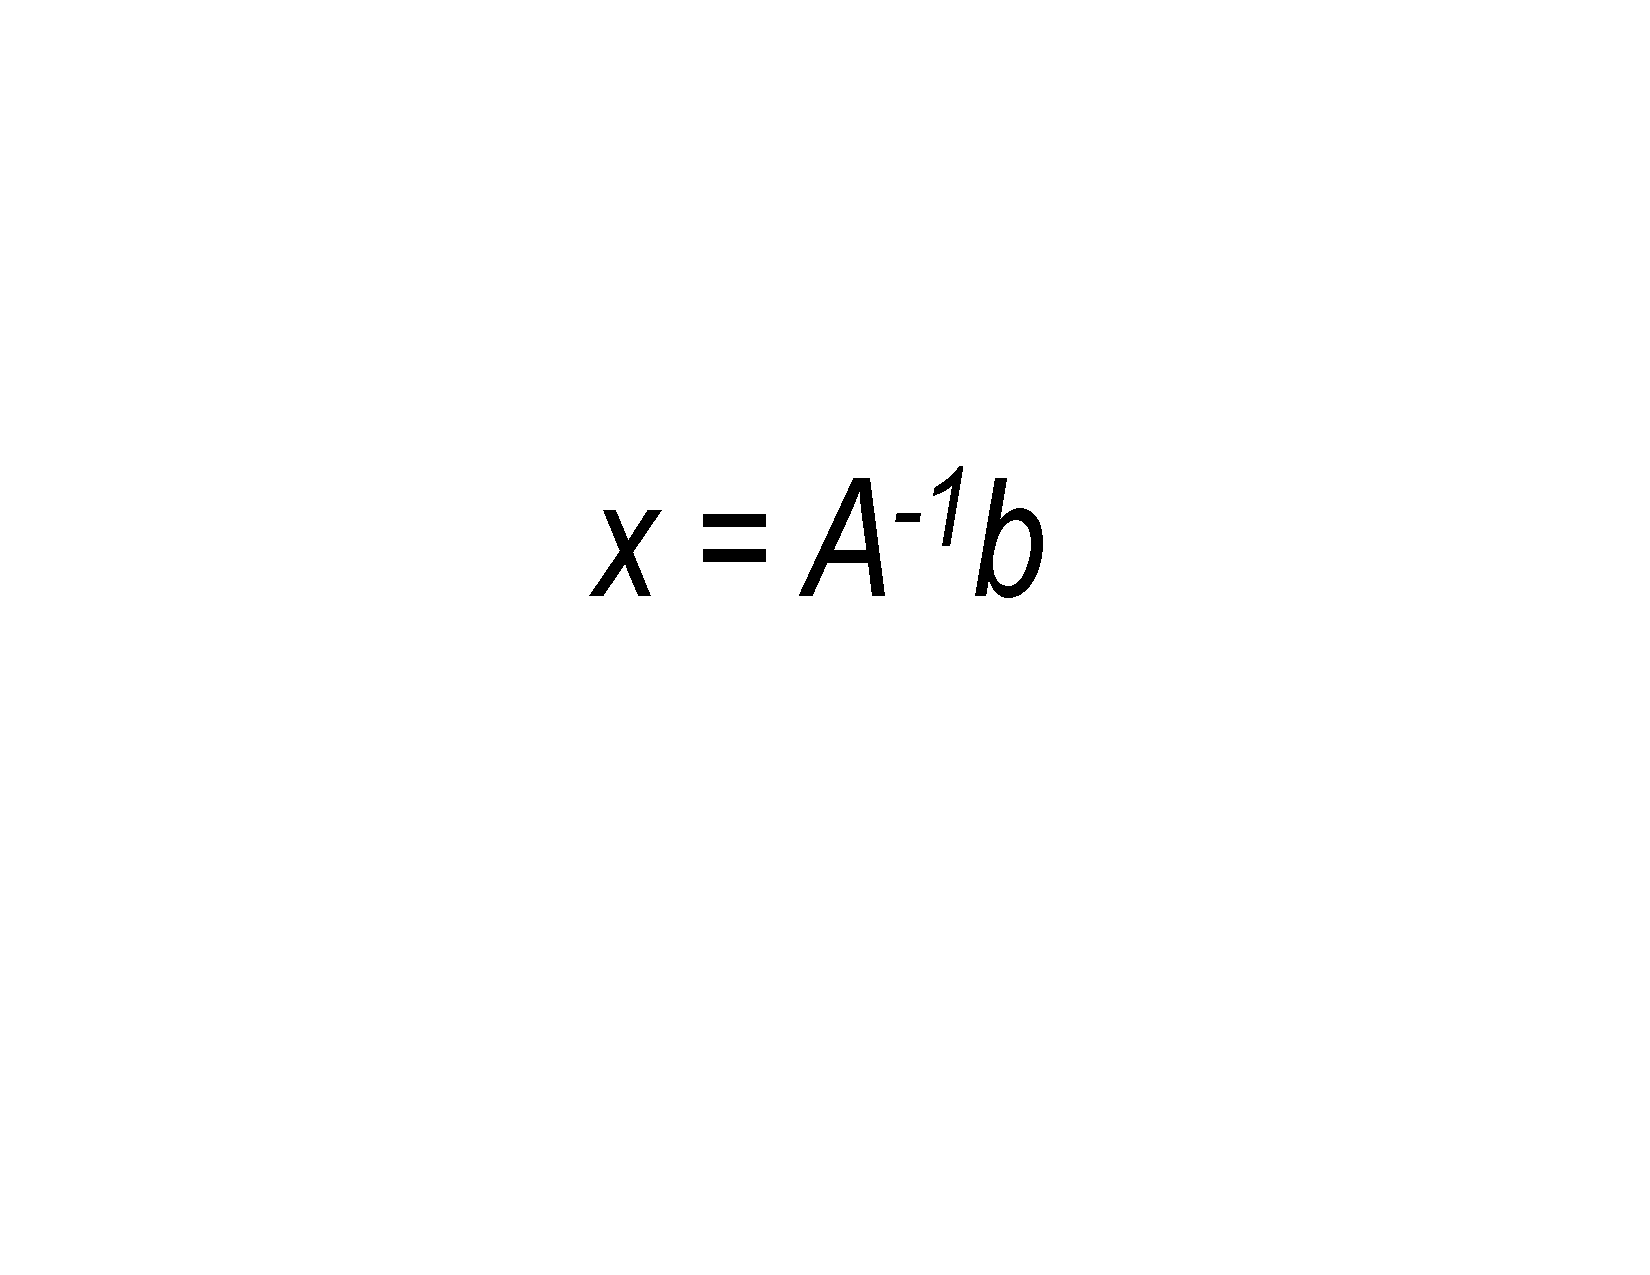
\includegraphics[scale=0.4]{../figures/naive1} \\[2ex]
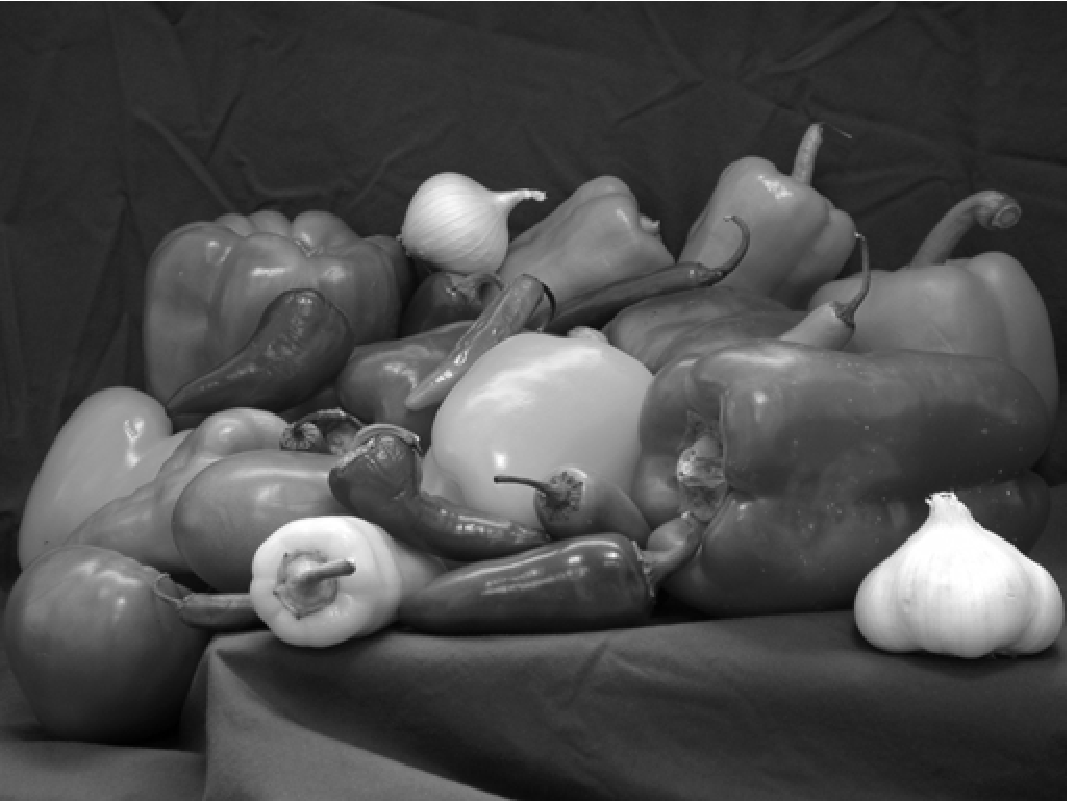
\includegraphics[scale=0.2]{../figures/fig1} \,
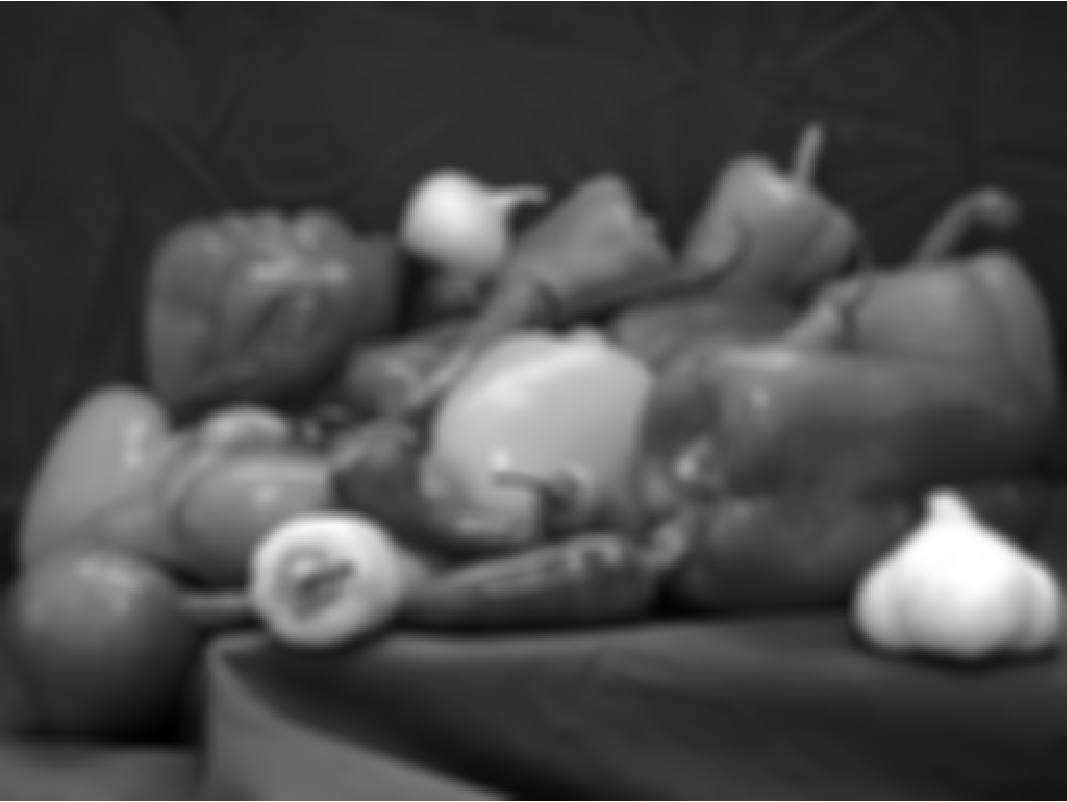
\includegraphics[scale=0.2]{../figures/fig2} \,
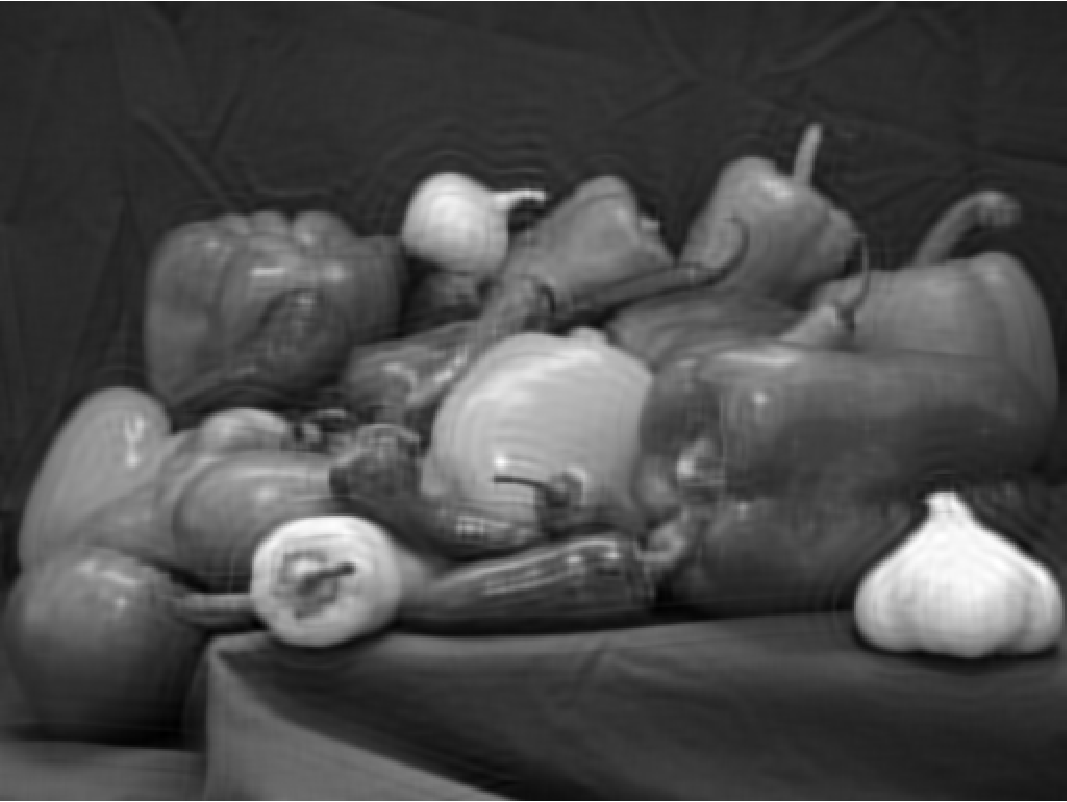
\includegraphics[scale=0.2]{../figures/fig3} \\
\small{\hspace{1em} True image \hspace{4em} Blurred image \hspace{3em} Recovered image}
\end{figure}
\end{frame}

\begin{frame}{Naive Solution}
\begin{figure}
\centering
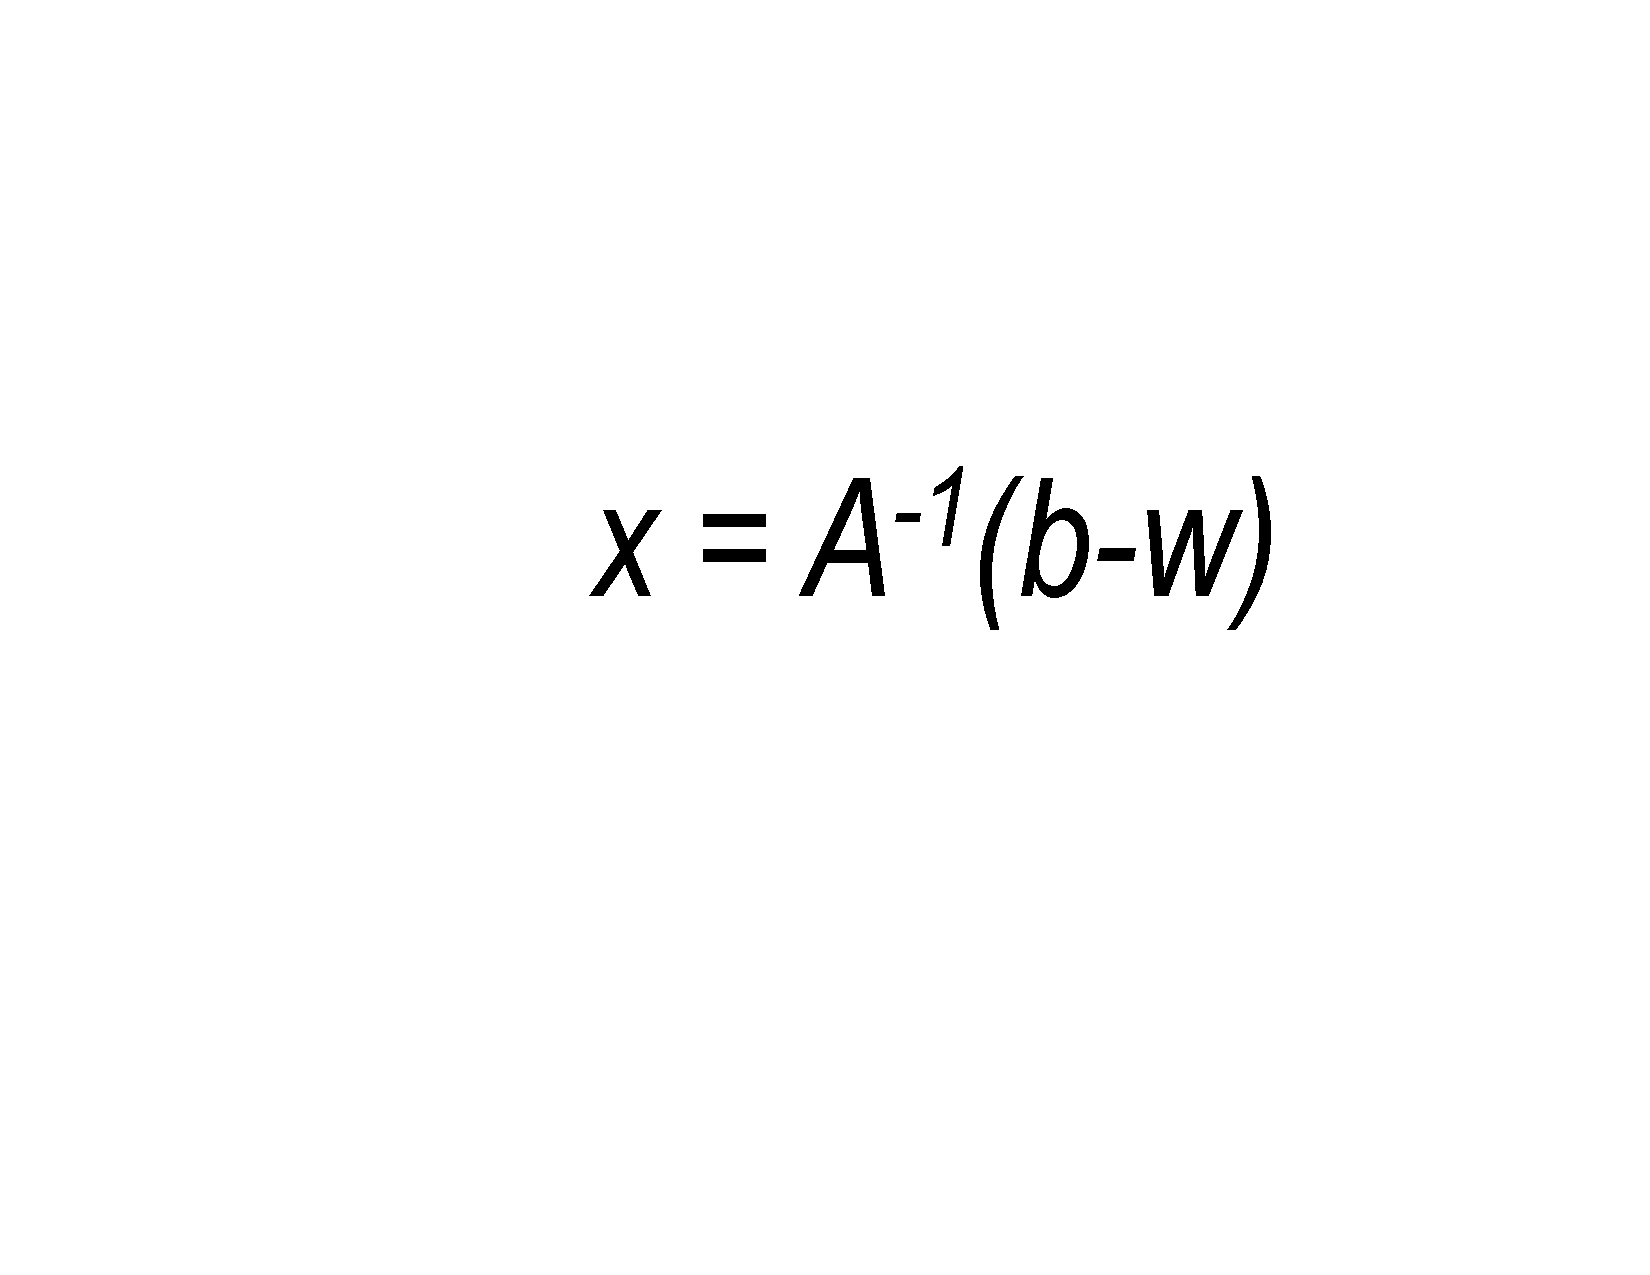
\includegraphics[scale=0.4]{../figures/naive2} \\[2ex]
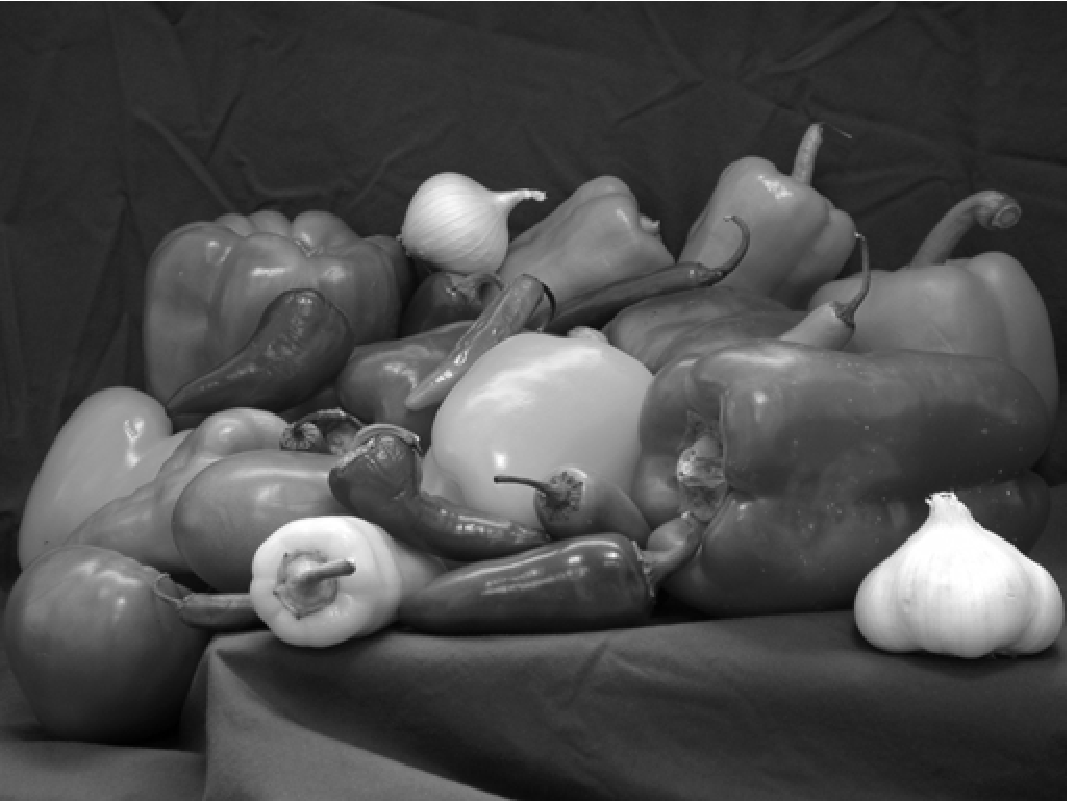
\includegraphics[scale=0.2]{../figures/fig1} \,
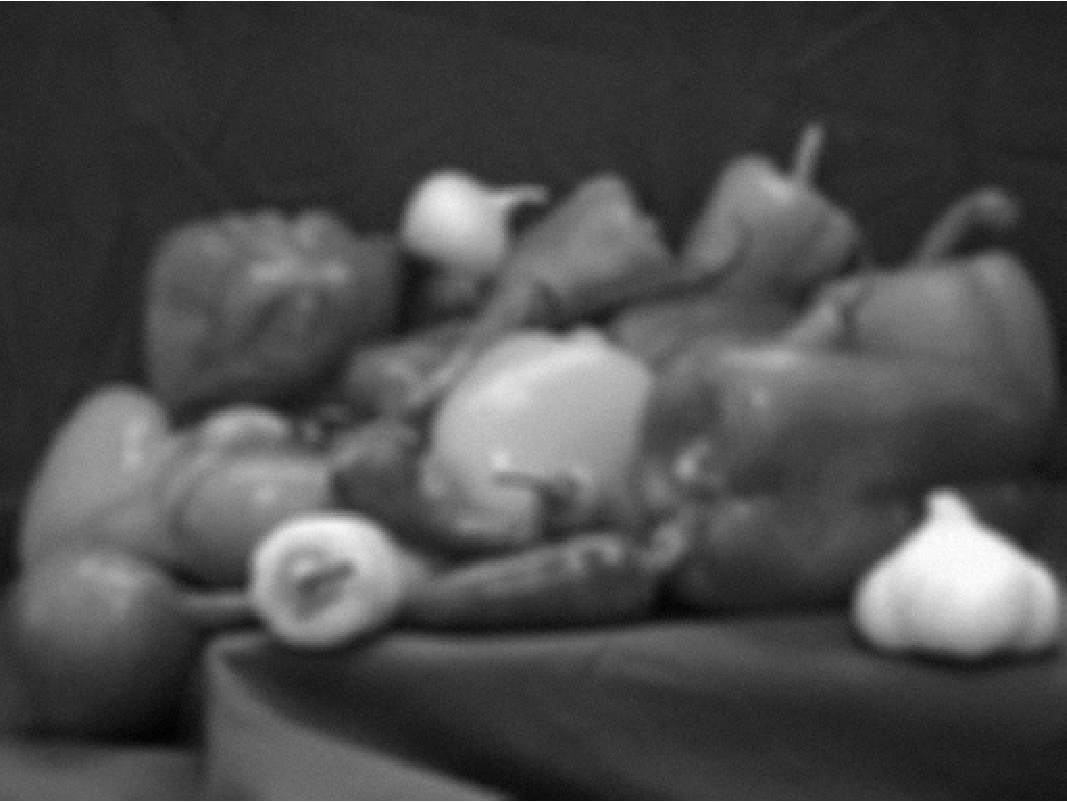
\includegraphics[scale=0.2]{../figures/fig4} \,
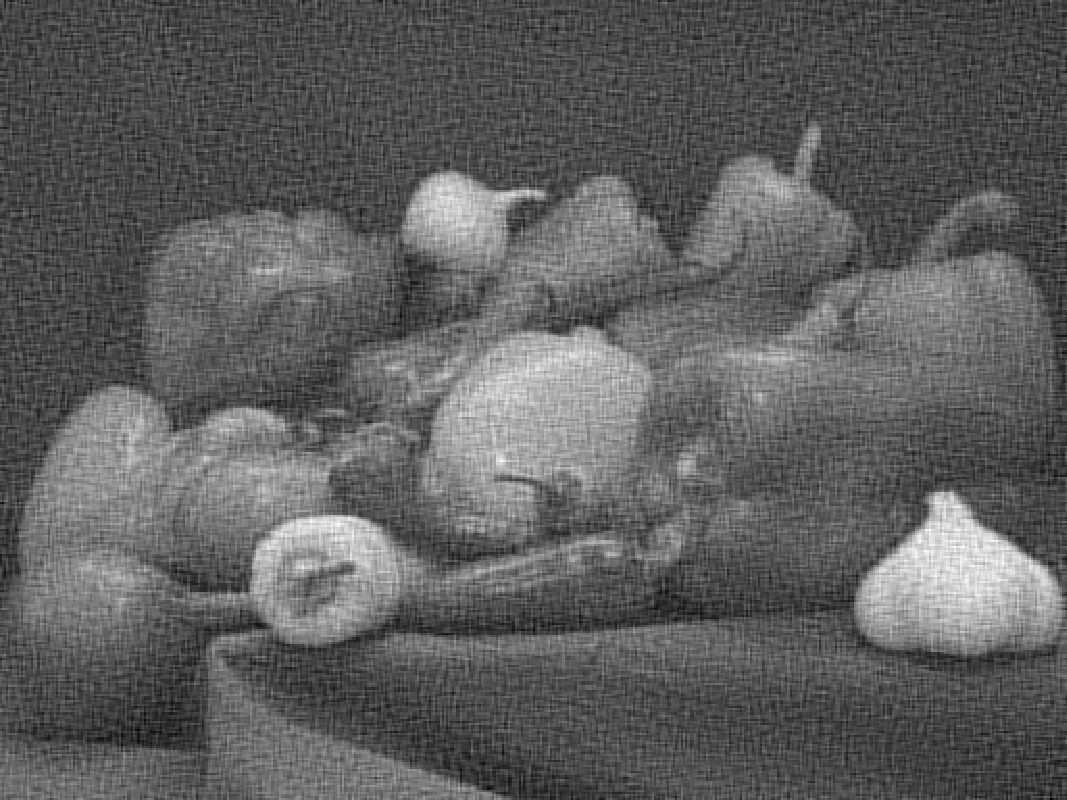
\includegraphics[scale=0.2]{../figures/fig5} \\
\small{\hspace{1em} True image \hspace{2em} Blurred and noisy image \hspace{1em} Recovered image}
\end{figure}
\end{frame}

% OBJECTIVE FUNCTIONS
\section{De(noise/blur)ing Objective Functions}

% Better Solution
\begin{frame}
Since the naive solution is contaminated by round-off error and noise, a better approach is to solve the problem:
\begin{block}{}
\[ \min_x \quad \underbrace{f(Ax-b)}_{\text{Fidelity term}}  \quad + \underbrace{\lambda R(x)}_{\text{Regularization}} \]
\end{block}

\begin{columns}[T]
	\begin{column}{0.45\linewidth}
		\begin{block}{Fidelity Term} \vspace{-2.5ex}
			\[ f = \left\{ \begin{matrix*}[l] 
			\| \cdot \|_F^2 \\[1ex] h_{\gamma}( \cdot ) \\[1ex] \gamma^{-1} \log(\cosh(\gamma \cdot)) 
			\end{matrix*} \right. \]
		\end{block}
	\end{column}
	\begin{column}{0.45\linewidth}
		\begin{block}{Regularization Term}
			\[ R = \left\{ \begin{matrix*}[l]
			TV(x) \\[1ex] \| Wx \|_1
			\end{matrix*} \right. \]
		\end{block}
	\end{column}
\end{columns}
\end{frame}

%\begin{frame}{A General Loss Function}
%
%$$
%L_b(x) = \underbrace{f(Ax-b)}_{\text{Fidelity Term}} + \underbrace{\lambda g(x)}_{\text{Noise Regularization}} + \underbrace{\delta(x | [0,1])}_{\text{Range of Pixel Values}}
%$$
%
%\begin{exampleblock}{Fidelity Term}
%\vspace{-5 mm}
%\begin{align*}
%f &= \left\{ \begin{aligned}
%&\|\cdot \|_F^2 \\
%& h_\gamma (\cdot)\\
%& \gamma^{-1} \log ( \cosh (\gamma \cdot ))
%\end{aligned}\right.
%\end{align*}
%\end{exampleblock}
%
%\begin{exampleblock}{Regularization Term}
%\vspace{-5 mm}
%\begin{align*}
%g &= \left\{ \begin{aligned}
%&TV(x) \\
%& \| Wx\|_1
%\end{aligned}\right.
%\end{align*}
%\end{exampleblock}
%
%\end{frame}

% Fidelity Term
\begin{frame}{Fidelity Term Penalty Functions}
\begin{minipage}{0.45\textwidth}

\begin{center}
\vspace{-2 mm}

\includegraphics[scale=0.35]{../figures/gaussian_noise.png} \\

\includegraphics[scale=0.35]{../figures/student_t_noise.png} 
\end{center}

\end{minipage} \hfill
\begin{minipage}{0.52\textwidth}

What is Ax - b
Why use different functions than frobenius norm?  Use pictures as motivation. Show quadratic and huber penalty functions, show different distributions?

\end{minipage}
\end{frame}

% Regularizers
\begin{frame}{Image Assumptions and Regularizers}
Either assume image is sparse in wavelet domain, or assume image is smooth

Talk about choice of g
Haar, FFT
What is TV?

Show two different definitions of TV from paper.
\end{frame}

% OPTIMIZATION WITH WAVELET REGULARIZATION
\section{Optimization with Wavelet Regularization}

\begin{frame}{Kelsey's stuff here}
\begin{itemize}
\item Loss function
\item choice of lambda
\item choice of wavelet
\item prox gradient method
\end{itemize}

\end{frame}

% OPTIMIZATION WITH TOTAL VARIATION REGULARIZATION
\section{Optimization with Total Variation Regularization}

\begin{frame}{Total Variation Regularization}

\begin{exampleblock}{Loss Function}
$$
L_b(x) = f(Ax-b) + \lambda \|x\|_{TV} + \delta(x | [0,1])
$$
\end{exampleblock}

\begin{exampleblock}{Proximal Gradient Step}
\begin{align*}
x^{k+1} &= \prox_{\mathcal{L}^{-1}(\lambda \|\cdot \|_{TV} + \delta_{[0,1]})} (\underbrace{x^k - \mathcal{L}^{-1} A^T\nabla f (Ax^k - b)}_{u^k}) \\
&= \AMz \left( \|u^k - z\|_F^2 + \lambda \|z\|_{TV} + \delta(z | [0,1]) \right) \\
&= P_{[0,1]}  \left( \AMz \left( \|u^k - z\|_F^2 + \lambda \|z\|_{TV} \right) \right)
\end{align*}
\end{exampleblock}

\end{frame}

\begin{frame}{Dual Form of Total Variation}

\begin{exampleblock}{A Few Definitions}
weee
\end{exampleblock}

\begin{exampleblock}{Total Variation}
blarg
\end{exampleblock}

\end{frame}

\begin{frame}{Dual Form of TV Denoising with $\|\cdot \|_F^2$}

\end{frame}

\begin{frame}{Optimization of Dual Form}

\begin{exampleblock}{Problem Statement}
\vspace{-5 mm}
\begin{align*}
&\underset{(p,q) \in \mathcal{P} }{\text{min}}  \left\{  \norm{b - \lambda \mathcal{L} (p,q)}_F^2 - \norm{(I-P_{[0,1]}) (b - \lambda \mathcal{L} (p,q))}_F^2   \right\}\\
&\underset{(p,q) }{\text{min}}  \left\{  \underbrace{\norm{b - \lambda \mathcal{L} (p,q)}_F^2 - \norm{(I-P_{[0,1]}) (b - \lambda \mathcal{L} (p,q))}_F^2}_{= h(p,q)} + \delta((p,q) | \mathcal{P})   \right\}
\end{align*}
\end{exampleblock}

\begin{exampleblock}{}
\begin{align*}
&\nabla h (p,q) = -2\lambda \mathcal{L}^TP_{[0,1]} (b - \lambda \mathcal{L}(p,q)) \\
&\text{Lipschitz with constant } \leq 16\lambda^2\\
&\Rightarrow \text{ Use projected gradient}
\end{align*}
\end{exampleblock}

\end{frame}

\begin{frame}{Optimization in Dual Form}

\begin{exampleblock}{Projection onto $\mathcal{P}$}
Recal $\mathcal{P} = (p,q) \in [-1,1]^{m-1 \times n}\times[-1,1]^{m \times n-1}$
\begin{align*}
P_\mathcal{P}(p,q) &= (r,s) \text{ with } \left\{ \begin{aligned}
r_{ij} &= sgn(p_{ij} ) \min \{ 1, |p_{ij}| \}\\
s_{ij} &= sgn(q_{ij} ) \min \{ 1, |q_{ij}| \}\\
\end{aligned}\right.
\end{align*}
\end{exampleblock}

\begin{exampleblock}{Projected Gradient Step}
\begin{align*}
(p^{k+1},q^{k+1} ) &= P_\mathcal{P} \left((p^k, q^k) + \frac{1}{8\lambda} \mathcal{L}^TP_{[0,1]} (b - \lambda \mathcal{L}(p,q)) \right)
\end{align*}
\end{exampleblock}

\end{frame}

\begin{frame}{Summary of Fast TV Regularization}
\begin{spacing}{1.6}
\fontsize{9}{10}\selectfont
\hspace{-3 mm}
\begin{minipage}{0.4\textwidth}
\textbf{MFISTA$(b,f, \lambda)$}
\begin{algorithmic}
\State $y^1 = x^0 = b; \, t^1 = 1$
\State $\alpha \geq Lip(\nabla f)$
\For {$k = 1:N$}
	\State $u^k = y^k - \frac{A^T\nabla f (A y^k - b)}{\alpha}$
	\State $z^k = FGP(u^k, \frac{\lambda}{2 \alpha})$
	\State $x^k = \underset{x \in \{x^{k-1},z^k\}}{\text{argmin}} \,L_b(x)$
	\State $t^{k+1} = \frac{1 + \sqrt{1 + 4{t^k}^2}}{2}$ 
	\State $y^{k+1} = x^k + \frac{t^k}{t^{k+1}}(z^k - x^k)$ 
	\State \hspace{10 mm}$+ \frac{t^{k-1}}{t^{k+1}}(z^k - x^k) $
\EndFor
\end{algorithmic}
\end{minipage}
\begin{minipage}{0.6\textwidth}

\textbf{FGP$(b, \lambda)$}
\begin{algorithmic}
\State $(r_{ij}^1, s_{ij}^1) = (p_{ij}^0, q_{ij}^0) = 0; \, t^1 = 1$
\For {$k = 1:N$}
	\State $(p^k,q^k) = P_\mathcal{P} \left( (r^k,s^k) - \frac{\mathcal{L}^TP_{[0,1]} (b - \lambda \mathcal{L}(r^k,s^k))}{8\lambda} \right)$
	\State $t^{k+1} = \frac{1 + \sqrt{1 + 4{t^k}^2}}{2}$ 
	\State $(r^k,s^k) = (p^k,q^k) + \frac{t^k-1}{t^{k+1}}(p^k-p^{k-1}, q^k-q^{k-1})$ 
\EndFor \\
\Return $P_{[0,1]} (b - \lambda \mathcal{L}(p^N,q^N))$
\end{algorithmic}

\end{minipage}
\end{spacing}
\end{frame}

\begin{frame}{Results: Gaussian Noise}
\begin{center}
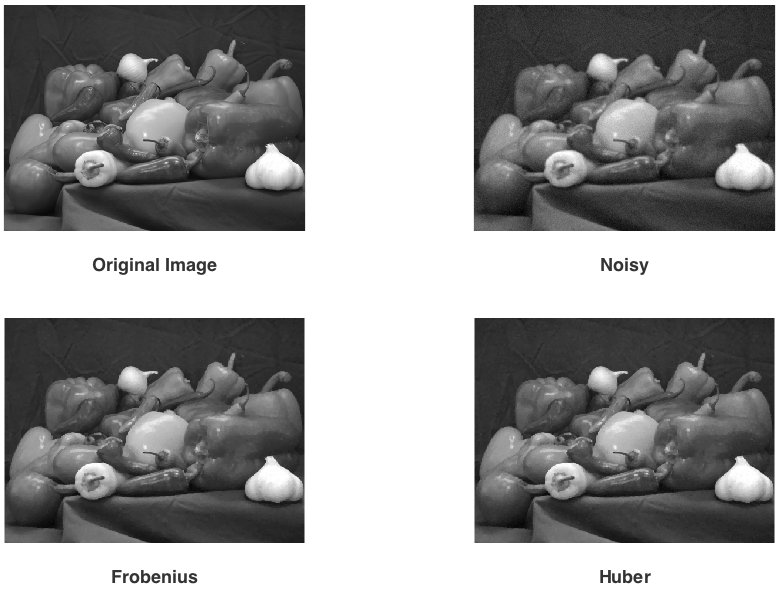
\includegraphics[scale=0.33]{gaussian_peppers.png} 
\end{center}
\end{frame}

\begin{frame}{Results: Students's-t Noise}

\end{frame}

\section{Discussion}

\section{Discussion}

\section*{References}
\begin{frame}{Questions?}
\begin{thebibliography}{10}    
\setbeamertemplate{bibliography item}[online]
\bibitem{code} Codes used to generate figures
\url{https://github.com/snagcliffs/Amath575project}

\beamertemplatebookbibitems % This gives it a nice book symbol
\bibitem{Guck} Guckenheimer, J., Holmes, P. \textit{Nonlinear Oscillations, Dynamical Systems, and Bifurcations of Vector Fields}. Springer-Verlag, 1983. Print.

\beamertemplatearticlebibitems % and an article symbol
\bibitem{brazil}  Oliveira, D., Leonel, E. (2008) \textit{Braz. J. Phys.} 38(1):62-64

\bibitem{corrdim} Grassberger, P., Procaccia, I. (1983) \textit{Phys. Rev. Letters.} 50(5):346-349

\end{thebibliography}
\end{frame}

\end{document}
